%-----------------------
% Title page
%-----------------------
\begin{titlepage}
  \centering

  \textsc{ELEC4630 Assignment 2}\\
  \vspace{9cm}

  \rule{\linewidth}{0.5pt}\\

  \vspace{1em}
  \LARGE\textsc{Question 3}\\
  \vspace{1em}

  \LARGE\uppercase{\textbf{{Face Recognition}}}\\

  \rule{\linewidth}{2pt}\\

  \vfill

  \normalsize{Deren Teo (4528554)}
  \vspace{1cm}

\end{titlepage}

%-----------------------
% Report body
%-----------------------
\section{Introduction}

The eigenface method is one of the more successful traditional face recognition techniques, and represents the first sufficiently effective method to enable automated face recognition \cite{rosebrock_2021}. Though the method is now obsolete, having been introduced in 1991, the eigenface method remained a baseline for face recognition for many years \cite{elec4630_2023}. This report presents an implementation of the eigenface method, and the results it achieves on a small data set of 33 faces.

\section{Background Theory}

\subsection{Principal Component Analysis}

Principal component analysis (PCA) is an unsupervised dimensionality reduction method which determines a set of orthogonal components that maximises the variance in the data \cite{alpaydin_2020} \cite{lovell_2008}. The method is unsupervised in that it does not use the output information \cite{alpaydin_2020}, only the covariance of the data \cite{lovell_2008}. The first principal component indicates the direction of largest variance, the second principal component the second largest variance, and so on \cite{alpaydin_2020}. Importantly, the orthogonality of the components means the resulting variances are uncorrelated \cite{alpaydin_2020}. PCA is frequently useful for data with high dimensionality, but where some or many features are highly correlated or otherwise not relevant to differentiating the data.

Mathematically, PCA is a linear transformation of the data into a coordinate space maximising variance along the pricipal components \cite{jolliffe_2002}. This is achieved by projecting the data onto the eigenvectors of the data covariance matrix, where the eigenvectors are ordered by their corresponding eigenvalues; the eigenvector with the largest corresponding eigenvalue defines the principal component \cite{rosebrock_2021}.

Consider the covariance matrix, $C$, of a data set with $N$ features. Matrix $C$ is square with size $N\times N$ \cite{lovell_2008}. An eigendecomposition of $C$ yields eigenvalues $\lambda_i$ and eigenvectors $u_i$, such that \cite{lovell_2008}:
\begin{align}
  C u_i = \lambda_i u_i,\ \forall i \in [1 \ldots N]
\end{align}

The number of eigenvalues and eigenvectors is at most equal to the number of samples in the data set. However, often a large proportion of variance is explained by the first few principal components. In these cases, the remaining principal components can be disregarded without incurring a significant reconstruction error.

Suppose the data set $D$ (of $N$ features) contains $n$ samples; $D$ may then be represented as a matrix of dimensions $n\times N$. Let the $m$ principal components with the largest corresponding eigenvalues be used to transform the data. This may or may not represent the entire set of eigenvectors, where $m=n$ in the first case and $m<n$ in the latter.

The data is transformed by projecting $D$ onto the space created by the $m$ eigenvectors \cite{rosebrock_2021}:
\begin{align}
  D'^{[n\times m]} = D^{[n\times N]} \cdot \begin{bmatrix} u_1 & u_2 & \cdots & u_m \end{bmatrix}^{[N\times m]}
\end{align}

Hence, the data dimensionality is reduced from $N$ to $m$ features, typically with $m<<N$.

\newpage
\subsection{Eigenfaces}

The eigenface method describes the application of PCA to the domain of face recognition \cite{lovell_2008}. Compared to standard PCA, the method of covariance matrix eigendecomposition differs to facilitate a tractable computation, which is necessary given the very large covariance matrices associated with the application of PCA to images \cite{lovell_2008}.

\subsection{Support Vector Machines}

\section{Methodology}

This section desribes the procedure used to develop a simple face recognition solution based on principal component analysis (PCA), also known as the eigenface method. Courtesy of abstraction libraries such as scikit-learn \cite{scikitlearn_2023}, PCA is almost trivial to implement. However, to assist in the understanding of the eigenface method, a description of the computations underlying the PCA steps are provided.

The following steps describe the procedure used to create a simple face recognition solution:

\begin{enumerate}
  \item The training and testing images are loaded into two separate sets and assigned a numeric label by face. The labels correspond to the folder enumeration in the data.

  \item All images are converted from 3-channel to single-channel greyscale in preparation for PCA.

  \item Each image is flattened into a single vector, and the training and testing images are stacked into two arrays of size $N\times(128\times128)$, where $N$ is the number of training or testing images, respectively.

  \item The scikit-learn library is used to create and fit a PCA model in one step. Internally, this involves:

  \begin{enumerate}
    \item ...

  \end{enumerate}

  \item The flattened images, both training and testing, are then transformed using the eigenvectors determined by PCA, reducing the dimensionality of each image from $128\times128=16,384$ to the number of eigenvectors, 6 in this case.

  \item A support vector machine (SVM) is trained to classify faces as a linear combination of the determined eigenfaces. The scikit-learn library enables this with a single command:

  \begin{center}
    \texttt{svm = sklearn.svm.SVC().fit(X\_train\_pca, y\_train)}
  \end{center}

  \item The SVM classifier is then applied to the testing images by predicting a label for each testing image.

\end{enumerate}

[Briefly explain SVM; classifies faces as linear combinations of eigenfaces]

\newpage
\section{Results}

The trained SVM classifier achieves a 97\% accuracy on the testing images, representing 32 out of 33 faces correctly recognised. The sole misidentification is presented in Figure \ref{fig:misidentification}.

\begin{figure}[ht]
  \centering
  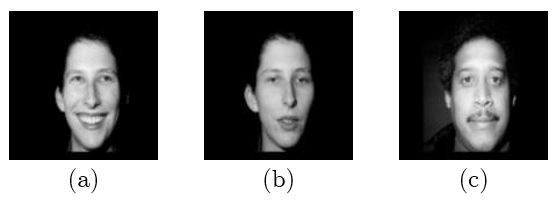
\includegraphics[width=0.6\textwidth]{images/q3_misidentification.png}
  \caption{Face 3a (a) is misidentified as individual 5. Training images of individual 3 (b) and 5 (c) are provided for reference.}
  \label{fig:misidentification}
\end{figure}

As an extension to the solution, a simple web-based GUI built using Gradio \cite{gradio_2023} was developed to enable a user to select an image from the testing set, and view the recognised image from the training set. Figure \ref{fig:gui} demonstrates the use of the GUI.

\begin{figure}[ht]
  \centering
  \begin{subfigure}[b]{0.8\textwidth}
    \centering
    
\includegraphics[width=\textwidth]{images/q3_gui_1.png}
    \caption{Landing screen}
  \end{subfigure}
  \\[1em]
  \begin{subfigure}[b]{0.8\textwidth}
    \centering
    
\includegraphics[width=\textwidth]{images/q3_gui_2.png}
    \caption{Image selected from testing set}
  \end{subfigure}
  \\[1em]
  \begin{subfigure}[b]{0.8\textwidth}
    \centering
    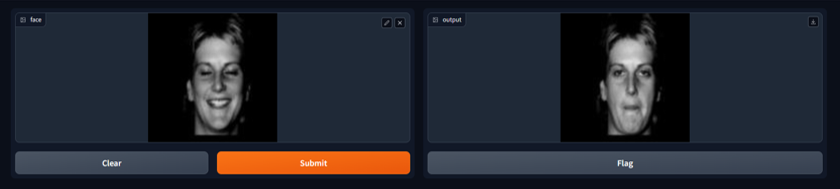
\includegraphics[width=\textwidth]{images/q3_gui_3.png}
    \caption{Recognised face produced from training set}
  \end{subfigure}
  \caption{A simple GUI built with Gradio, enabling a user to validate recognition results.}
  \label{fig:gui}
\end{figure}

\newpage
\section{Discussion}

This report has presented an implementation of the eigenface method of face recognition. The solution is trained on a set of six distinct faces, and achieves a 97\% accuracy rate in classifying the same six faces in a test set of 33 images with varying facial expression. The result represents 32 out of 33 faces correctly recognised, with the single error having been presented in the previous section.

\textit{Issues with eigenface techniques}
\begin{itemize}
  \item \textit{As quoted from literature}
  \item \textit{Try removing one face from the training set, to represent ``new'' face}
\end{itemize}

\section{Conclusion}
